\documentclass{beamer}
\usepackage[utf8]{inputenc}
\usepackage{palatino}
\usepackage{subfig}
\usepackage{amsmath}
\usepackage{dsfont}
\usepackage{multimedia}
\usepackage{hyperref}

\usetheme{Warsaw}
\usecolortheme{crane}

% www.sharelatex.com/learn/Beamer

\title{Computing Entropies with Nested Sampling}
\author{Brendon J. Brewer}
\institute{Department of Statistics\\
The University of Auckland}
\date{\color{blue}\url{https://www.stat.auckland.ac.nz/~brewer/}}

\begin{document}

\frame{\titlepage}


% New slide
\begin{frame}
\frametitle{What is entropy?}

Firstly, I'm talking about information theory, not thermodynamics (though the
two are connected).

\end{frame}


% New slide
\begin{frame}
\frametitle{Shannon entropy}

Consider a discrete probability distribution with probabilities
$\boldsymbol{p} = \{p_i\}$. The Shannon entropy is
\begin{align}
H(\boldsymbol{p}) &= -\sum_i p_i \log p_i
\end{align}

It is a real-valued property of the distribution.

\end{frame}



% New slide
\begin{frame}
\frametitle{Relative entropy}

Consider two discrete probability distributions with probabilities
$\boldsymbol{p} = \{p_i\}$ and $\boldsymbol{q} = \{q_i\}$.
The relative entropy is
\begin{align}
H(\boldsymbol{p}; \boldsymbol{q}) &= -\sum_i p_i \log\left(\frac{p_i}{q_i}\right)
\end{align}
Without the minus sign,
it's the `Kullback-Leibler divergence', and is more fundamental than the
Shannon entropy. With uniform $\boldsymbol{q}$, it reduces to the Shannon
entropy (up to an additive constant).
\end{frame}


% New slide
\begin{frame}
\frametitle{Entropy quantifies uncertainty}
If there are just $N$ equally likely possibilities,
i.e., $p_i = 1/N$, then $H = \log N$. \vspace{0.5em}

\begin{center}
\includegraphics[width=0.6\textwidth]{entropy1.pdf}
\end{center}

\end{frame}


% New slide
\begin{frame}
\frametitle{Entropy quantifies uncertainty}
If there are just $N$ equally likely possibilities,
i.e., $p_i = 1/N$, then $H = \log N$. \vspace{0.5em}

\begin{center}
\includegraphics[width=0.6\textwidth]{entropy2.pdf}
\end{center}

\end{frame}

% New slide
\begin{frame}
\frametitle{Entropy quantifies uncertainty}
If there are just $N$ equally likely possibilities,
i.e., $p_i = 1/N$, then $H = \log N$. \vspace{0.5em}

\begin{center}
\includegraphics[width=0.6\textwidth]{entropy3.pdf}
\end{center}

\end{frame}


% New slide
\begin{frame}
\frametitle{What about densities?}
We get `differential entropy'

\begin{align}
H = - \int_{\textnormal{all }x} f(x) \log f(x) \, dx
\end{align}

This generalises log-volume, as defined {\bf with respect to} $dx$.

\begin{alertblock}{Important}
Differential entropy is {\em coordinate-system dependent}.
\end{alertblock}

\end{frame}



% New slide
\begin{frame}
\frametitle{Statements and questions}
Consider a problem with three mutually exclusive, exhaustive possibilities
\texttt{a}, \texttt{b}, and \texttt{c}.


\begin{center}
  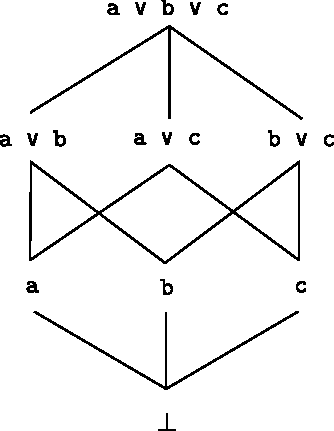
\includegraphics[width=0.3\textwidth]{lattice1.pdf}
\end{center}

\end{frame}



% New slide
\begin{frame}
\frametitle{Some entropies in Bayesian statistics}
Writing them in terms of parameters $\boldsymbol{\theta}$ and data
$d$, for Bayesian purposes.

\begin{enumerate}
\item Entropy of the prior for the parameters $H(\boldsymbol{\theta})$
\item Entropy of the conditional prior for the data $H(\boldsymbol{\theta} | d)$
\item Entropy of the posterior $H(\boldsymbol{\theta} | d)$
\item Entropy of the prior for the data $H(d)$
\end{enumerate}

Note: {\em conditional entropies} such as (2) and (3)
are defined using an expectation over the quantity conditioned upon.

\end{frame}


% New slide
\begin{frame}
\frametitle{Connections}

Entropy of the joint prior:
\begin{align}
H(\boldsymbol{\theta}, d) &= H(\boldsymbol{\theta}) + H(d | \boldsymbol{\theta}) \\
                          &= H(d) + H(\boldsymbol{\theta} | d).
\end{align}

Mutual information:
\begin{align}
I(\boldsymbol{\theta}; d) &= H(\boldsymbol{\theta}) - H(\boldsymbol{\theta} | d).
\end{align}
This quantities dependence --- or more fundamentally,
relevance, or the potential for learning.

\end{frame}




% New slide
\begin{frame}
\frametitle{References I.}

On the connection between Shannon entropy and thermodynamic entropy,
see: \vspace{2em}

{\tiny Jaynes, Edwin T. ``Gibbs vs Boltzmann entropies.''
American Journal of Physics 33, no. 5 (1965): 391-398. \\

Brewer, Brendon J. ``Unscrambling the Second Law of Thermodynamics''
{\color{blue}
  \url{https://quillette.com/2016/01/28/unscrambling-the-second-law-of-thermodynamics}
}
} % tiny

\end{frame}



\end{document}


